% !Rnw weave = knitr
% !TEX TS-program = lualatex
% !TEX encoding = UTF-8 Unicode

\documentclass{article}\usepackage[]{graphicx}\usepackage[]{color}
%% maxwidth is the original width if it is less than linewidth
%% otherwise use linewidth (to make sure the graphics do not exceed the margin)
\makeatletter
\def\maxwidth{ %
  \ifdim\Gin@nat@width>\linewidth
    \linewidth
  \else
    \Gin@nat@width
  \fi
}
\makeatother

\definecolor{fgcolor}{rgb}{0.345, 0.345, 0.345}
\newcommand{\hlnum}[1]{\textcolor[rgb]{0.686,0.059,0.569}{#1}}%
\newcommand{\hlstr}[1]{\textcolor[rgb]{0.192,0.494,0.8}{#1}}%
\newcommand{\hlcom}[1]{\textcolor[rgb]{0.678,0.584,0.686}{\textit{#1}}}%
\newcommand{\hlopt}[1]{\textcolor[rgb]{0,0,0}{#1}}%
\newcommand{\hlstd}[1]{\textcolor[rgb]{0.345,0.345,0.345}{#1}}%
\newcommand{\hlkwa}[1]{\textcolor[rgb]{0.161,0.373,0.58}{\textbf{#1}}}%
\newcommand{\hlkwb}[1]{\textcolor[rgb]{0.69,0.353,0.396}{#1}}%
\newcommand{\hlkwc}[1]{\textcolor[rgb]{0.333,0.667,0.333}{#1}}%
\newcommand{\hlkwd}[1]{\textcolor[rgb]{0.737,0.353,0.396}{\textbf{#1}}}%
\let\hlipl\hlkwb

\usepackage{framed}
\makeatletter
\newenvironment{kframe}{%
 \def\at@end@of@kframe{}%
 \ifinner\ifhmode%
  \def\at@end@of@kframe{\end{minipage}}%
  \begin{minipage}{\columnwidth}%
 \fi\fi%
 \def\FrameCommand##1{\hskip\@totalleftmargin \hskip-\fboxsep
 \colorbox{shadecolor}{##1}\hskip-\fboxsep
     % There is no \\@totalrightmargin, so:
     \hskip-\linewidth \hskip-\@totalleftmargin \hskip\columnwidth}%
 \MakeFramed {\advance\hsize-\width
   \@totalleftmargin\z@ \linewidth\hsize
   \@setminipage}}%
 {\par\unskip\endMakeFramed%
 \at@end@of@kframe}
\makeatother

\definecolor{shadecolor}{rgb}{.97, .97, .97}
\definecolor{messagecolor}{rgb}{0, 0, 0}
\definecolor{warningcolor}{rgb}{1, 0, 1}
\definecolor{errorcolor}{rgb}{1, 0, 0}
\newenvironment{knitrout}{}{} % an empty environment to be redefined in TeX

\usepackage{alltt}
\usepackage[utf8]{inputenc}
\usepackage[english, georgian]{babel}
\usepackage{fontspec}
\usepackage{geometry, graphicx}
 % you must load Sweave with the `noae` option
\setmainfont[
Extension=.ttf,
UprightFont={*},
BoldFont = {arial_geo-bold},
ItalicFont = {arial_geo-italic},
BoldItalicFont = {arial_geo-bold-italic}
]{arial_geo}

\usepackage{hyperref}
\hypersetup{
    colorlinks=true,
    linkcolor=blue,
    filecolor=magenta,      
    urlcolor=cyan,
}

\title{ლაბორატორული სამუშაო 1: შესავალი R-გარემოში}
\author{დავით სიჭინავა}
\date{\today}
\IfFileExists{upquote.sty}{\usepackage{upquote}}{}
\begin{document}



% \SweaveOpts{concordance=TRUE}
\maketitle
\section*{თემები}
\begin{itemize}
\item შესავალი R-გარემოში
\item R-ის მომხმარებლის გრაფიკული გარემო: R-Studio
\item R-ის მომხმარებლის გრაფიკული გარემოს ძირითადი ელემენტები
\item R-მარკირების დოკუმენტის შექმნა
\item ,,წიგნიერი პროგრამირება'' და პროექტების ორგანიზების კარგი პრაქტიკა 
\end{itemize}

\section*{ინსტრუქცია:}

თანმიმდევრობით შეასრულეთ მითითებული ამოცანები. თქვენს .rmd ფაილს სახელწოდება მიანიჭეთ შემდეგი ფორმით: თქვენი გვარი\_lab1.rmd. მაგალითად:

\begin{knitrout}
\definecolor{shadecolor}{rgb}{0.969, 0.969, 0.969}\color{fgcolor}\begin{kframe}
\begin{alltt}
\hlstd{sichinava_lab1.Rmd}
\end{alltt}
\end{kframe}
\end{knitrout}

\section*{დავალებები:}

\subsection*{ფაილების სისტემა და ნავიგაცია:}

პირველ რიგში, შექმენით სამუშაო დირექტორია თქვენს კომპიუტერში. რახან ამ კურსის ფარგლებში თითქმის ყოველი ლექციის შემდეგ პრაქტიკული სამუშაოა გათვალისწინებული, შექმენით კურსისთვის ცალკე ფოლდერი, სახელად intro\_stats\_r. ამ ფოლდერში დაამატეთ ქვე-ფოლდერი lab\_1, სადაც პირველი ლაბორატორიული სამუშაოს მასალებს შეინახავთ.

\begin{figure}[h]
\centering
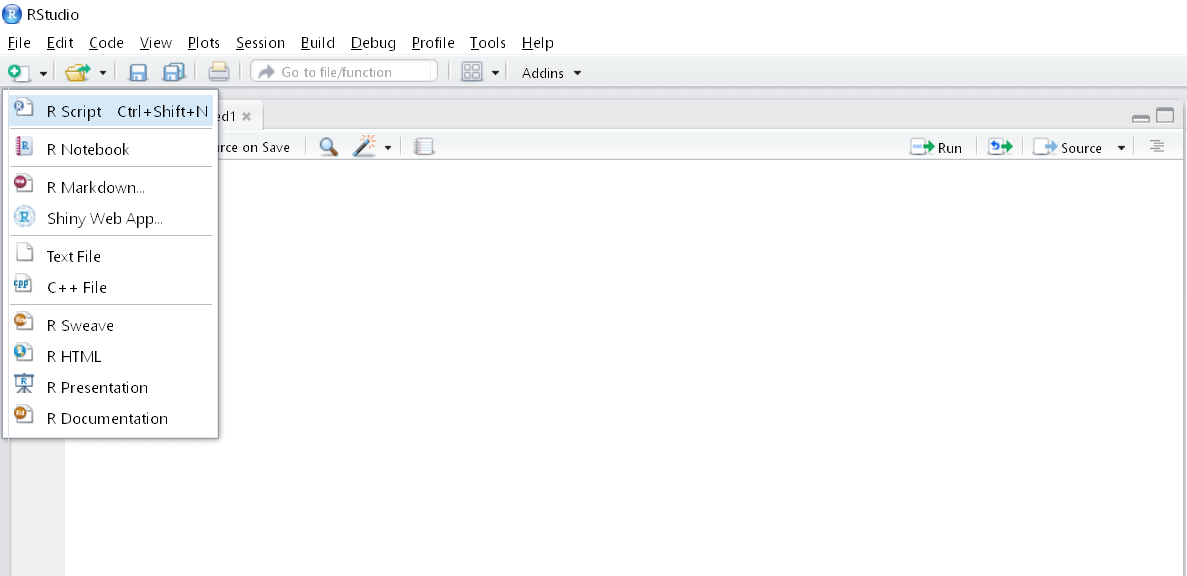
\includegraphics[width=\textwidth]{img/new_menu.PNG}
\caption{ახალი ფაილის შექმნა}
    \label{create:file}
\end{figure}

გახსენით R-Studio და შექმენით R-ბლოკნოტის ახალი ფაილი. დაარქვით სახელი და შეინახეთ lab\_1 ფოლდერში. შეგახსენებთ, რომ ფაილის შექმნა შესაძლებელია მენიუს შესაბამის ელემენტზე დაწკაპუნებით და სასურველი ტიპის ფაილის არჩევით (სურ. \ref{create:file}).




შესანიშნავია! ახლა ბლოკნოტის დასაწყისში, პრეამბულის შემდეგ (იხ. სურათი \ref{preamble}) აკრიფეთ მცირე ტექსტი R-studio-ზე თქვენი პირველი შთაბეჭდილებების შესახებ. ორი ან სამი წინადადება საკმარისია.

\begin{figure}[h]
\centering
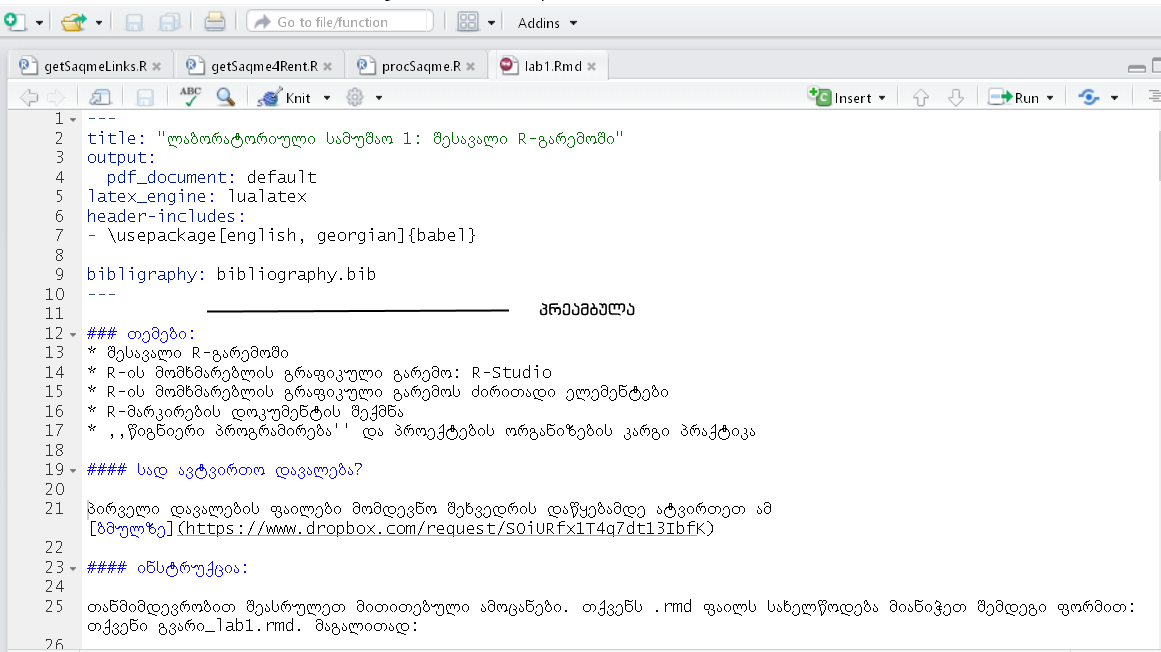
\includegraphics[width=\textwidth]{img/preamble.PNG}
\caption{დოკუმენტის პრეამბულა}
    \label{preamble}
\end{figure}

R-ბლოკნოტში ჩასვით კოდის ნაწილის აღმნიშვნელი მარკერები. დარწმუნდით, რომ თქვენი კოდი აქტიურია, რისთვისაც დააჭირეთ მარჯვენა კუთხეში მდებარე მწვანე სამკუთხა ღილაკს (იხ. სურ. \ref{chunk}). აქცენტის ნიშნებს შორის მიუთითეთ სინტაქსი, რომლის მეშვეობითაც თქვენს სამუშაო დირექტორიაში გადაინაცვლებთ.


ბიბლიოთეკების ჩამოტვირთვა და გამოძახება

R-ბლოკნოტში ჩასვით კოდის ახალი ნაწილი. ჩაწერეთ სინტაქსი, რომელიც ჩამოტვირთავს ბიბლიოთეკას ggplot2. გაუშვით სინტაქსი და დარწმუნდით, რომ იგი მუშაობს.

ახალ კოდის ნაწილში მიუთითეთ სინტაქსი, რომელიც ggplot2 ბიბლიოთეკას გაააქტიურებს. წინა დავალების მსგავსად, გაუშვით და შეამოწმეთ, ყველაფერი რიგზეა თუ არა.

\subsection*{ სკრიპტის ფაილის შექმნა და მისი ბლოკნოტში შემოტანა}

დააჭირეთ ახალი ფაილის შექმნის ღილაკს და აირჩიეთ R სკრიპტის ფაილი. გაითვალისწინეთ, რომ სკრიპში მუშაობისას, ტექსტის ჩვეულებრივად მითითება არ ხდება. თუ სიტყვიერი ახსნის ჩაწერა გჭირდებათ, მაშინ ტექსტის წინ დიეზის ნიშანი უნდა ჩაწეროთ და კოდი ,,გააკომენტაროთ'' (იხ. სურ. \ref{comment}). ასეთ კოდს პროგრამა შესრულებისას უგულებელყოფს.

\begin{figure}[h]
\centering
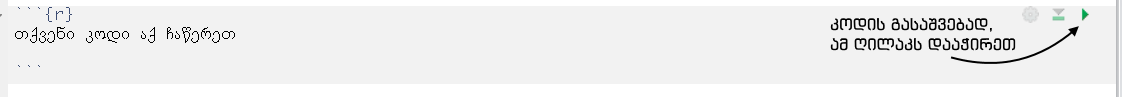
\includegraphics[width=\textwidth]{img/run_chunk.PNG}
\caption{კოდის ნაწილის მითითება და გაშვება}
    \label{chunk}
\end{figure}


სკრიპტის ფაილში ჩაწერეთ სინტაქსი, რომელიც tidyr ბიბლიოთეკას ჩამოტვირთავს და გაააქტიურებს. სკრიპტის ფაილი სამუშაო დირექტორიაში, სპეციალური ქვეფოლდერში "source" შეინახეთ და ლოგიკური სახელი მიანიჭეთ.

წიგნიერი პროგრამირების წესებით რომ ვიმოქმედოთ, საჭიროა, სკრიპტის ფაილი ბლოკნოტიდან გავუშვათ. ამისთვის დაუბრუნდით ბლოკნოტს, ჩასვით ახალი კოდის ნაწილი, ჩაწერეთ სკრიპტის გასაშვები სინტაქსი და შეასრულეთ.

\subsection*{დოკუმენტის საბოლოო გაფორმება}

წიგნიერი პროგრამირების პრინციპების კიდევ ერთხელ დაცვის მიზნით, თითოეულ კოდის ნაწილს მიუწერეთ მცირე აღწერა, თუ რა ფუნქციას ასრულებს. ტექსტის გაფორმებისთვის გამოიყენეთ მარკირების ენის მრავალფეროვანი შესაძლებლობები. მაგალითად, გამოყავით სექციები, ჩასვით ბმულები, სურათები. ტექსტი გააფორმეთ კურსივით და მსხვილი ასოებით და ა. შ. მარკირების ენის დეტალური დოკუმენტაცია \href{https://www.rstudio.com/wp-content/uploads/2016/03/rmarkdown-cheatsheet-2.0.pdf}{ამ} და  \href{https://github.com/adam-p/markdown-here/wiki/Markdown-Cheatsheet}{ამ} ბმულზე შეგიძლიათ, ნახოთ.

\begin{figure}[h]
\centering
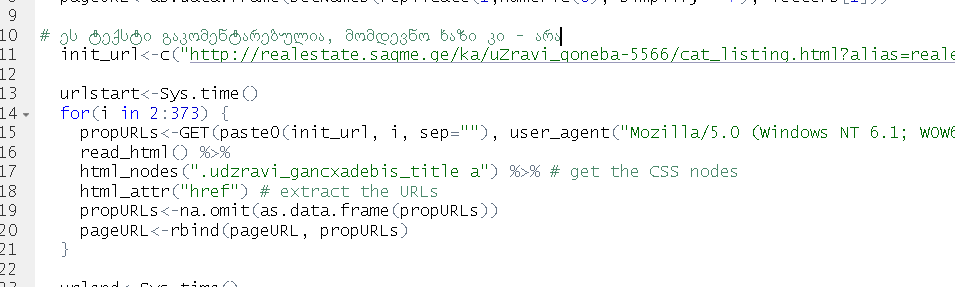
\includegraphics[width=\textwidth]{img/commented.PNG}
\caption{კოდის გაკომენტარება}
    \label{comment}
\end{figure}



\subsection*{დოკუმენტის კომპილაცია}

კომპილაციამდე (ე.ი. მარკირების html ფორმატში გადატანამდე) შეინახეთ თქვენი ბლოკნოტი. html ანუ ჰიპერტექსტების მარიკრების ენის დოკუმენტი ნებისმიერი ვებსაიტის საფუძველია - ნებისმიერი ვებგვერდი, რასაც თქვენს ბროუზერში ხედავთ, html-დოკუმენტების ერთობლიობას წარმოადგენს. R-ბლოკნოტი მარკირების შემდეგ ცალკე html-დოკუმენტად იქცევა, რომლის გახსნა ნებისმიერი, შედარებით თანამედროვე ბროუზერის მეშვეობითაა შესაძლებელი.

\begin{figure}[h]
\centering
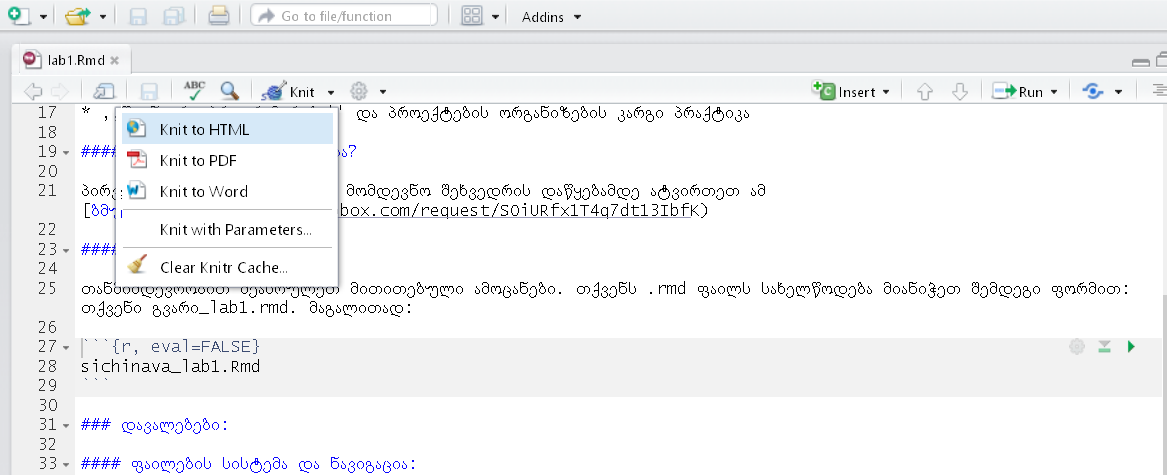
\includegraphics[width=\textwidth]{img/knit_to_html.PNG}
\caption{ბლოკნოტის კომპილაცია}
    \label{compile}
\end{figure}


ბლოკნოტის კომპილაციისთვის დააჭირეთ ძაფის გორგლის ფორმის ღილაკს და აირჩიეთ ბრძანება \emph{knit to HTML} (იხ. სურ. \ref{compile}. თუ ყველაფერი სწორად გააკეთეთ, მზა დოკუმენტი ავტომატურად გაიხსნება. გახსოვდეთ, რომ კომპილაციის დროს, R-Studio კოდის ნაწილებში მითითებულ სინტაქსსაც ასრულებს.

\subsection*{ანოტირებული ბიბლიოგრაფია}

რახან მარკირების ენის გარკვეულ საფუძვლებს უკვე ვფლობთ, ანოტირებული ბიბლიოგრაფიის ტექსტიც R-ბლოკნოტის საშუალებით მოამზადეთ. ამისთვის თქვენს კომპიუტერში დააყენეთ ტექსტური რედაქტორი (მაგალითად, Notepad++), შენახული ბლოკნოტის ფაილი მისი მეშვეობით გახსენით და ანოტაციის ტექსტი ჩაწერეთ. ანოტირებული ბიბლიოგრაფიისთვის APA ციტირების სტილი და შემდეგი შაბლონი გამოიყენეთ, იმ განსხვავებით, რომ თქვენი ტექსტი ქართულად უნდა იყოს:

\\

Waite, L. J., Goldschneider, F. K., & Witsberger, C. (1986). Nonfamily living and the erosion of traditional family orientations among young adults. American Sociological Review, 51, 541-554

\emph{The authors, researchers at the Rand Corporation and Brown University, use data from the National Longitudinal Surveys of Young Women and Young Men to test their hypothesis that nonfamily living by young adults alters their attitudes, values, plans, and expectations, moving them away from their belief in traditional sex roles. They find their hypothesis strongly supported in young females, while the effects were fewer in studies of young males. Increasing the time away from parents before marrying increased individualism, self-sufficiency, and changes in attitudes about families. In contrast, an earlier study by Williams cited below shows no significant gender differences in sex role attitudes as a result of nonfamily living.}


(მაგალითი აღებულია შემდეგი ვებსაიტიდან: http://guides.library.cornell.edu/annotatedbibliography)

მას შემდეგ, რაც ტექსტს მორჩებით, დაიმახსოვრეთ, დახურეთ Notepad++, ბლოკნოტი R-Studio-ს მეშვეობით გახსენით და დააკომპილირეთ.

\subsection*{მოვრჩი. როგორ ჩავაბარო ჩემი ნამუშევარი?}

თქვენს მიერ შექმნილი დირექტორია დააარქივეთ (.zip ან .rar ფორმატში). მიღებულ ფაილს სახელი შემდეგი ფორმატით დაარქვით: გვარი\_lab1.zip. მაგალითდ:
\begin{knitrout}
\definecolor{shadecolor}{rgb}{0.969, 0.969, 0.969}\color{fgcolor}\begin{kframe}
\begin{alltt}
\hlstd{sichinava_lab1.zip}
\end{alltt}
\end{kframe}
\end{knitrout}

მიღებული ფაილი მომდევნო შეხვედრის დაწყებამდე ატვირთეთ ამ \href{https://www.dropbox.com/request/oUc9abSj2pWwLHgObGV7}{ბმულზე} ან ამ მისამართზე: https://goo.gl/ss9XmR




\end{document}
